\documentclass[DIV=15]{scrartcl}


\usepackage{graphicx}
\usepackage{epstopdf} 
\usepackage{amsfonts,amsmath,enumerate,amssymb,bm,siunitx}
\usepackage[numbers]{natbib}



\begin{document}

\section*{Within-Host Stuff}

The within-host dynamics are governed by these equations:
\begin{gather*}
\frac{\text{d} \bm{x}}{ \text{d} t} = (1-k)Q \bm{x} + ar_L \bm{y}-\bm{x} \big((1-k)\bar{\gamma} + a r_L \big), \\
\frac{\text{d} \bm{y}}{ \text{d} t} = \frac{k}{r_L}Q \bm{x} - a \bm{y}-\bm{y} \bigg(\frac{k}{r_L}\bar{\gamma} - a \bigg),
\end{gather*}
where $Q=( q_{ij}) = (m_{ij}\gamma_{ij})$ is the replication-mutation matrix.  $r_L$ is the relative reservoir size, 
$k$ is the rate of entering the reservoir and $a$ the  rate of leaving it. (Also what is $\gamma$?). $\bm{x}$ and $\bm{y}$ are the frequencies of each strain in the active compartment and the reservoir respectively.

\subsection*{PrEP: No Reservoir}
First two strains only are considered: resistant and wild-type.  The fitnesses of the two  strains (replication rates)  are then given by \begin{equation}
\gamma (t) = \begin{pmatrix}
1.05(1- C(t)) \\1
\end{pmatrix} , 
\label{gamma}
\end{equation}
where $C(t)$ is relative concentration of the drug (i.e $C=1$ means it is completely effective and $C=0$ has no effect). For now the drug profile is taken to  be as in Figure \ref{drug}(a). So the person goes onto PrEP shortly after having contracted HIV (at $t=0$) after $6$ months (REF) they are taken of it. It is assumed that at $t=2$ they receive proper treatment (ART).
\begin{figure*}[h]
 \begin{center}$
 \begin{array}{cc}
 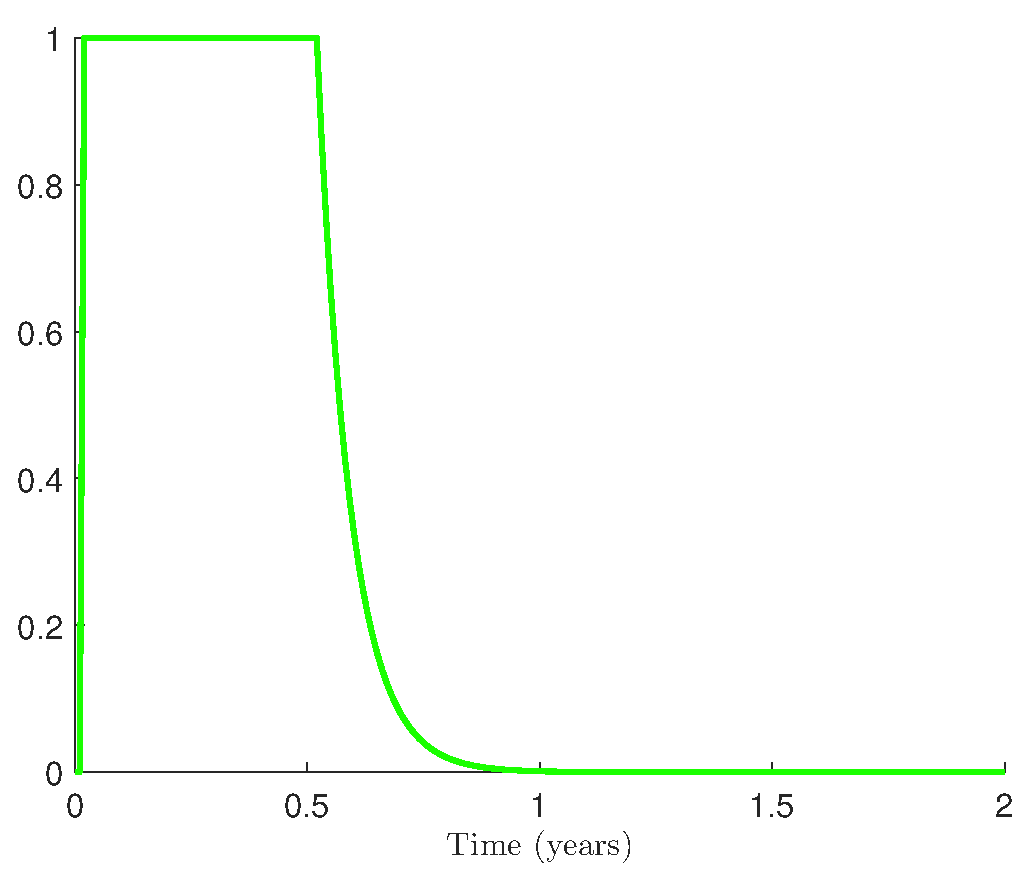
\includegraphics[width=.35\linewidth]{DrugConc_19_04a.eps} &
 \includegraphics[width=.35\linewidth]{WithinHost_20_04b.eps}
 \end{array}$
 \end{center}
	\caption{The concentration of drug and the effect on the replication rate of the virus. A bigger fitness difference or different action of drug might be needed, what is realistic?}
\label{drug} 
\end{figure*}

 Without the reservoir the frequency of the resistant strain  is $0.001$  at $t=2$, so it  makes up  $0.1 \%$ of the bad stuff. At equilibrium we will have A frequency of about $0.0002$, due to the mutations I suppose (this needs to be checked properly).
 % it's still at $0.001$ at $t=10$.
 Figure \ref{drug}(b) shows how the  fitness is affected by the drug. This needs better justification and stuff.
\begin{figure*}[h]
 \begin{center}$
 \begin{array}{cc}
 \includegraphics[width=.35\linewidth]{WithinHost_20_04a.eps} &
 \includegraphics[width=.35\linewidth]{WithinHost_21_04a.eps}
 \end{array}$
 \end{center}
 \caption{The within-host dynamics in the  absence of the reservoir. The mutation probability is $\SI{5e-5}{}$ per replication and $ \gamma $ is as in equation (\ref{gamma}).}
 \label{freqwithoutres}
 \end{figure*}
 One would hope that the frequency is low enough at $t=2$ that any extra mutations are unlikely to happen.
 
 \subsection*{PrEP: Reservoir}

For a large range of parameter values the presence of the reservoir increases the amount of resistant strain in the active compartment. It is assumed that the founder strain is the wild-type so this may be preferentially passed on (REF), so this may need to be accounted for. Also find what is considered to be the most appropriate amount of time to wait until going onto ART and how quickly PrEP is removed from body after treatment ends.
\begin{figure*}[h]
 \begin{center}$
 \begin{array}{cc}
 \includegraphics[width=.35\linewidth]{FrequencyofResistantStraininActiveCompartment_20_04a.jpg} &
 \includegraphics[width=.35\linewidth]{FrequencyofResistantStraininActiveCompartment_20_04b.jpg}
 \end{array}$
 \end{center}
 \caption{Increase in frequency of  the resistant strain present in the active compartment due to the presence of the reservoir. In the left image the homoeostatic proliferation rate is zero ($k = r_L a$). In the right we have $a = 0.01$. With the drug concentration and reproduction rate as before.}
 \label{freqwithres}
 \end{figure*}
Figure \ref{freqwithres} show the increase in frequency of the resistant strain compared to what happens without reservoir.  So it mostly tends to increase the frequency and the effect could be increased by changing around the drug concentration and the time that the person goes onto ART. So do this! Look at Figure \ref{freqwithres just 1} for dynamics in worst case with the above parameters.


\begin{figure*}[h]
 \begin{center}$
 \begin{array}{cc}
 \includegraphics[width=.35\linewidth]{WithinHostActive_20_04a.eps} &
 \includegraphics[width=.35\linewidth]{WithinHostReservoir_20_04a.eps}
 \end{array}$
 \end{center}
 \caption{Strain frequencies in the active compartment and the reservoir for $k = 0.0051$, $a = 0.01$ and $r_L = 2$. The other parameters are the same as before.}
 \label{freqwithres just 1}
 \end{figure*}
 
\section*{Between  Host}
To model  the between host effects more than one host type needs to  be considered. Now there are $n$ strains and $m$ host types, so the equations are (see \cite{Lythgoe2013}): 
\begin{gather}
H^{(j)}_{i}(t) = \frac{S^{(j)}(t)}{N(t)}  \sum_{k=1}^n \sum_{l=1}^m  \int_0^{T^{(l)}_{k}} \alpha^{(j)}_{k}(\tau) x^{(l)}_{ik}(\tau) H^{(l)}_{k}(t-\tau)e^{-\mu \tau} \ \text{d}\tau \label{multi1} \\
I_i^{(j)}(t) = \int_0^{T_i^{(j)}}  H_i^{(j)}(t-\tau)e^{-\mu \tau} \  \text{d}\tau \\
S(t) = N(t) -  \sum_{k=1}^n \sum_{l=1}^m  I^{(l)}_k(t) \\
\frac{\text{d}}{\text{d} t}  N(t) = B- \mu N(t) -\sum_{k=1}^n \sum_{l=1}^m  H_k^{(l)}(t-T_k^{(l)})e^{-\mu T_k^{(l)}}
\end{gather}
$H^{(j)}_{i}(t)$ is the rate infections initiated with strain $i$ occur in host type $j$. This bit might not be correct but it is assumed that $S(t) =  \sum_{l=1}^m S^{(l)}$. In the simple case there are a fixed proportion of susceptibles of each host type so in equation(\ref{multi1}) $S^{(j)}$ would be replaced by  a constant $c_j$. Is this the way to do it? The infectivity profile now depends on the host being infected so in this form $\beta_{ij}$ cannot be expressed explicitly. The infectivity profiles are in Figure  \ref{Infectivity}
\begin{figure*}[h]
 \begin{center}$
 \begin{array}{cc}
 \includegraphics[width=.35\linewidth]{Infectivity1_20_04a.eps} &
 \includegraphics[width=.35\linewidth]{Infectivity2_20_04a.eps}
 \end{array}$
 \end{center}
 \caption{The infectivity profiles for each host type. In the absence of the drug the wild type is more  infectious, but it will not infect people on PrEP. For this the set point viral load for  the wild-type  is \SI{1e4}{} and the resistant strain SPVL is chosen relative to this.}
 \label{Infectivity}
 \end{figure*}




\iffalse
also have different $x$s for each host type, $x_{ij}$ is frequency of strain $i$ in active compartment originally infected with strain $j$, so in many host equations this need sto be how much virus is in infecting host, then it is multiplied by infectivity profile for host type being infected.




my with in host stuff seems to  work  the same as single host stuff as long as zeros  aren't put into the original good soo fitness and infectivity for all on prep or non on prep are 0.001 otherwise nans happen 

\fi



Initially assume that a proportion $p$ of susceptible population are on PrEP, so that  $S^{(1)}(t) = (1-p)S(t)$ and $S^{(2)}(t) = pS(t)$.  That is, for host type $1$ $C(t) = 0$ and for host type $2$ $C(t) = 1$. Using the reservoir parameters as in figure \ref{freqwithres} and mutation rate of $\SI{5e-5}{}$ the stuff in Figure \ref{20 on prep} is what happens
\begin{figure*}[h]
 \begin{center}$
 \begin{array}{cc}
 \includegraphics[width=.35\linewidth]{20ONPrEPFreq_21_04a.eps} &
 \includegraphics[width=.35\linewidth]{20ONPrEPSusInf_21_04a.eps}
 \end{array}$
 \end{center}
 \caption{Two host types: on PrEP and not on PREP (the proportion on PrEP is fixed at $20\%$).}
 \label{20 on prep}
 \end{figure*}

Increasing $p$ to $0.3 $ saves almost everyone (see Figure \ref{30 on prep}). Some kind of herd immunity thing, does this seem reasonable? Better parameters (more realistic) are needed. Also the resistant strain does not increase in frequency,  wrong? With this model with low numbers on PrEP the resistant won't find the right hosts and with lot on PrEP the replication rate is so low that mutations rarely occur? 
\begin{figure*}[h]
 \begin{center}$
 \begin{array}{cc}
 \includegraphics[width=.35\linewidth]{30ONPrEPFreq_21_04a.eps} &
 \includegraphics[width=.35\linewidth]{30ONPrEPSusInf_21_04a.eps}
 \end{array}$
 \end{center}
 \caption{Two host types: on PrEP and not on PREP (the proportion on PrEP is fixed at $30\%$).}
 \label{30 on prep}
 \end{figure*}


\iffalse
\begin{figure*}
% Use the relevant command to insert your figure file.
% For example, with the graphicx package use
  \includegraphics[width=0.75\textwidth]{WithinMultiHost.eps}
% figure caption is below the figure
\caption{within host dynamics for two host two strain system. Top  two are in host not on the drug, where blue is the wild type and red is  the resistant strain. In the bottom two the host is on PrEP,as we are dealing with frequencies initiating wth the wild type  in a host on pRep GIVES A FREQUENCY  of 1 for  the wild type  (but this is just relative) soitmay be good either to set the frequency to 0 if the actual amount is small enough (so it not add to 1) or the infectivity will need to take account of both the host transmitting the virus and the host getting it.}
\label{fig:noh}       % Give a unique label
\end{figure*}
\fi

\section*{Parameters 'n' that}
So far have just used 
\begin{equation*}
M =  \begin{pmatrix} 1-\SI{5e-5}{} & \SI{5e-5}{} \\ \SI{5e-5}{} & 1- \SI{5e-5}{} \end{pmatrix} \qquad \gamma(t) = \begin{pmatrix} 1.05(1- C(t)) \\1 \end{pmatrix}
\end{equation*}
where I should say what $C(t)$ is.

\begin{table}
% table caption is above the table
\caption{Parameters used for figures}
\label{tab:1}       % Give a unique label
% For LaTeX tables use
\begin{tabular}{c|c|c|c|c|c|c}
\hline\noalign{\smallskip}
{} & $a$ & $r_L$ & $k$ & $\mu$ & $B$ & $p$\\
\noalign{\smallskip}\hline\noalign{\smallskip}
Figure \ref{drug}(b) & $0$ & NA & $0$ & $0.02$ & $200$ & NA\\
Figure \ref{freqwithres} & $0.01$ & $2$ & $0.0051$ & $0.02$ & $200$ & NA \\
Figure \ref{20 on prep} & $0.01$ & $2$ & $0.0051$ & $0.02$ & $200$ & $0.2$ \\
Figure \ref{30 on prep} & $0.01$ & $2$ & $0.0051$ & $0.02$ & $200$ & $0.3$ \\
\noalign{\smallskip}\hline
\end{tabular}
\end{table}



\bibliographystyle{apa}
\bibliography{DTCProject1Bibliography}   % name your BibTeX data base



 
\end{document}